% --------------------------------------------------------------
% This is all preamble stuff that you don't have to worry about.
% Head down to where it says "Start here"
% --------------------------------------------------------------
 
\documentclass[12pt]{article}
 
\usepackage[margin=1in]{geometry} 
\usepackage{amsmath,amsthm,amssymb}
 \usepackage{graphicx, color}
\newcommand{\N}{\mathbb{N}}
\newcommand{\Z}{\mathbb{Z}}
 
\newenvironment{theorem}[2][Theorem]{\begin{trivlist}
\item[\hskip \labelsep {\bfseries #1}\hskip \labelsep {\bfseries #2.}]}{\end{trivlist}}
\newenvironment{lemma}[2][Lemma]{\begin{trivlist}
\item[\hskip \labelsep {\bfseries #1}\hskip \labelsep {\bfseries #2.}]}{\end{trivlist}}
\newenvironment{exercise}[2][Exercise]{\begin{trivlist}
\item[\hskip \labelsep {\bfseries #1}\hskip \labelsep {\bfseries #2.}]}{\end{trivlist}}
\newenvironment{reflection}[2][Reflection]{\begin{trivlist}
\item[\hskip \labelsep {\bfseries #1}\hskip \labelsep {\bfseries #2.}]}{\end{trivlist}}
\newenvironment{proposition}[2][Proposition]{\begin{trivlist}
\item[\hskip \labelsep {\bfseries #1}\hskip \labelsep {\bfseries #2.}]}{\end{trivlist}}
\newenvironment{corollary}[2][Corollary]{\begin{trivlist}
\item[\hskip \labelsep {\bfseries #1}\hskip \labelsep {\bfseries #2.}]}{\end{trivlist}}
 
\begin{document}
 
% --------------------------------------------------------------
%                         Start here
% --------------------------------------------------------------
 
%\renewcommand{\qedsymbol}{\filledbox}
 
\title{Programming Assignment 3}%replace X with the appropriate number
\author{Sneha Reddy Aenugu, EE11B059\\ %replace with your name
} %if necessary, replace with your course title
 
\maketitle

\section{Clustering}
 
\begin{itemize}
\item{For each of the below data, the visualizations are provided in Figures 1 - 7.


\begin{figure}
	\centering
		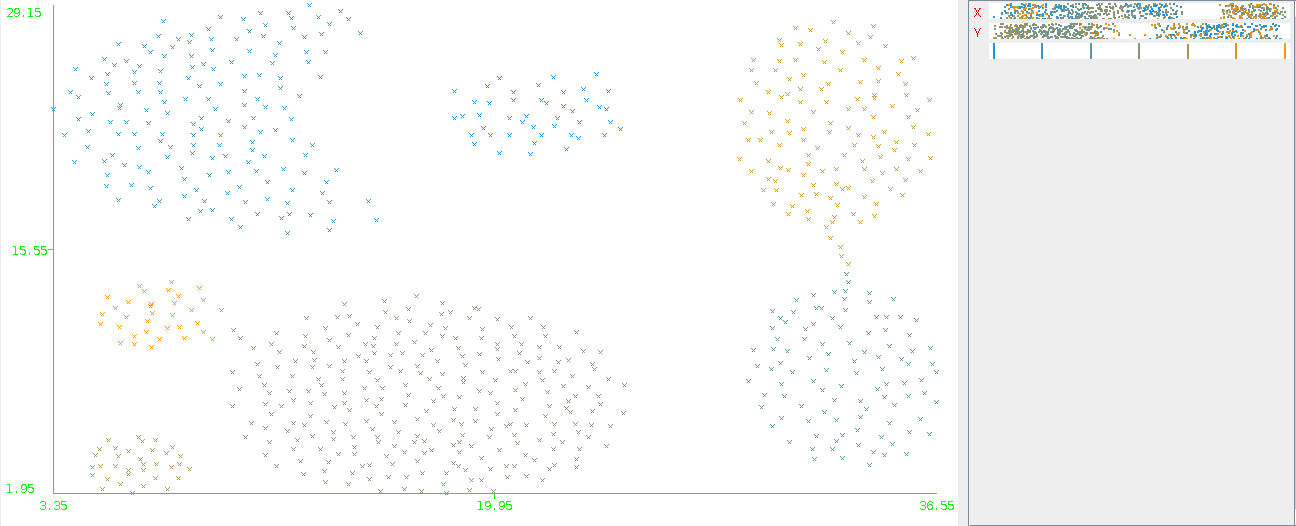
\includegraphics[scale = 0.4]{/home/sneha/Acads/9thsem/ML/P3/aggregation.png}
	\caption{Aggregation}
	
\end{figure}


\begin{figure}
	\centering
		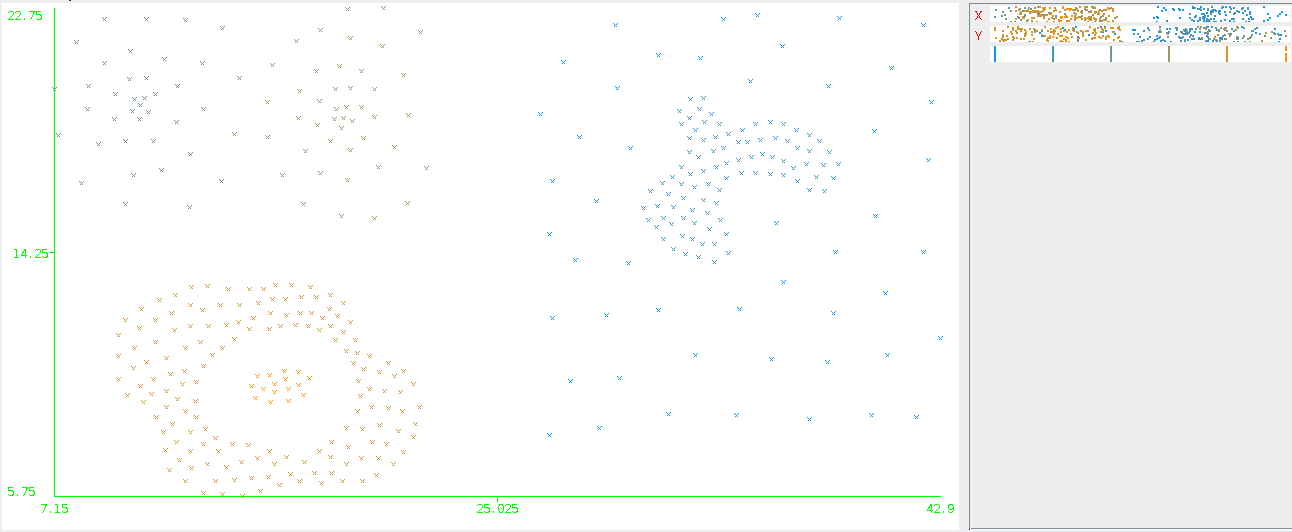
\includegraphics[scale = 0.4]{/home/sneha/Acads/9thsem/ML/P3/compound.png}
	\caption{Compound}
	
\end{figure}




\begin{figure}
	\centering
		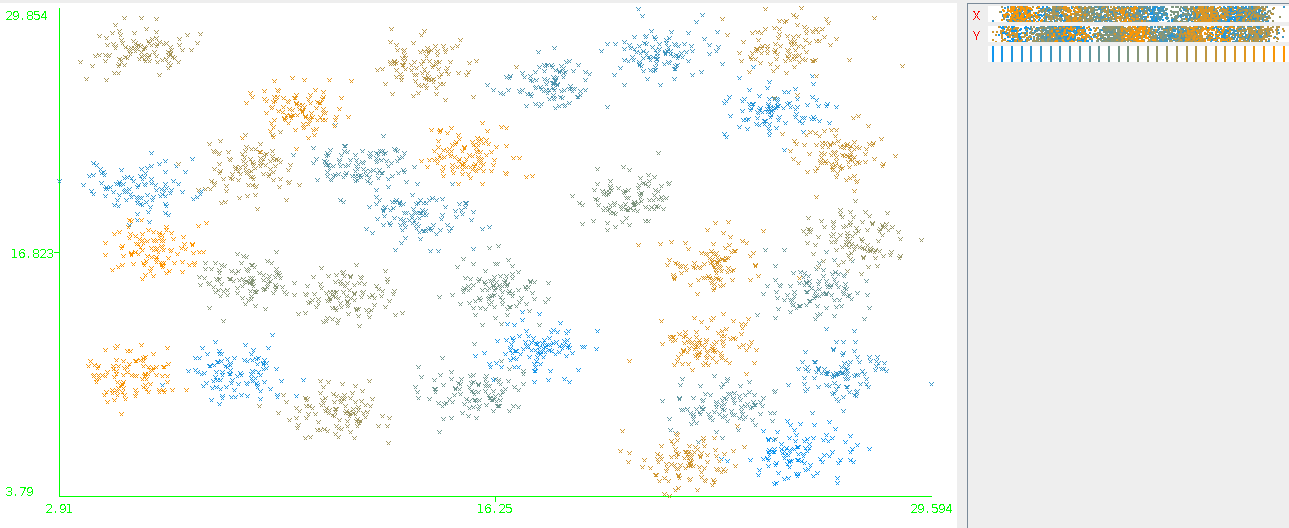
\includegraphics[scale = 0.4]{/home/sneha/Acads/9thsem/ML/P3/d31.png}
	\caption{D31}
	
\end{figure}


\begin{figure}
	\centering
		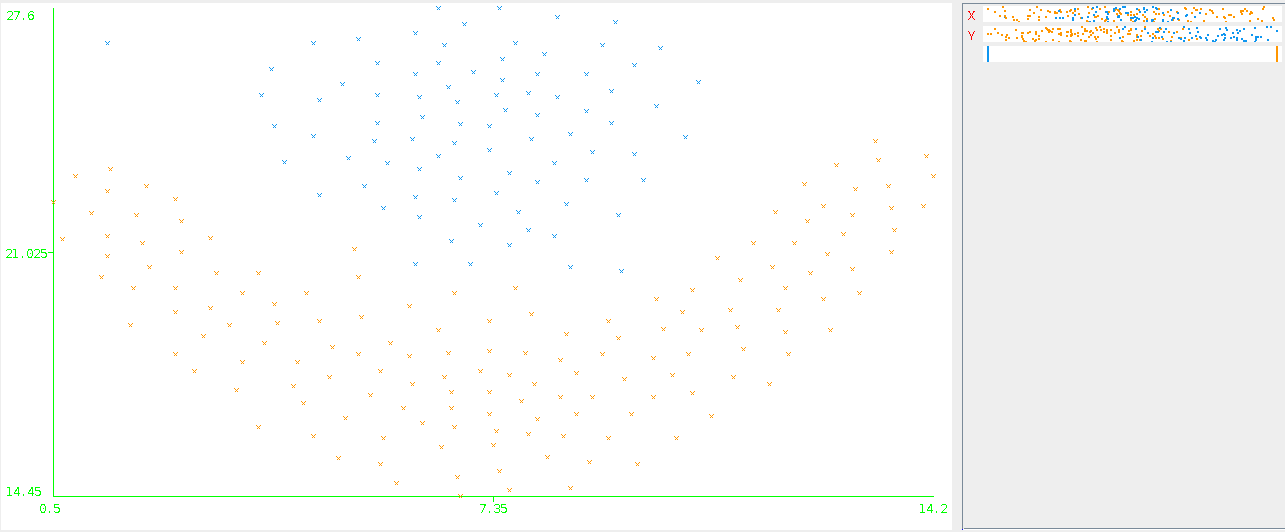
\includegraphics[scale = 0.4]{/home/sneha/Acads/9thsem/ML/P3/flames.png}
	\caption{Flames}
	
\end{figure}


\begin{figure}
	\centering
		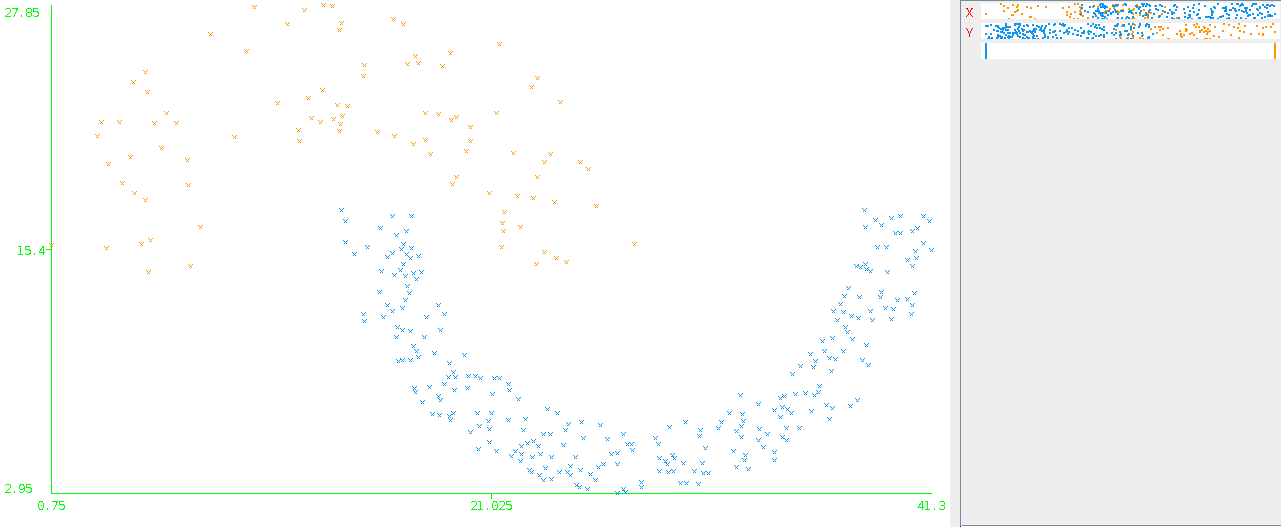
\includegraphics[scale = 0.4]{/home/sneha/Acads/9thsem/ML/P3/jain.png}
	\caption{Jain}
	
\end{figure}




\begin{figure}
	\centering
		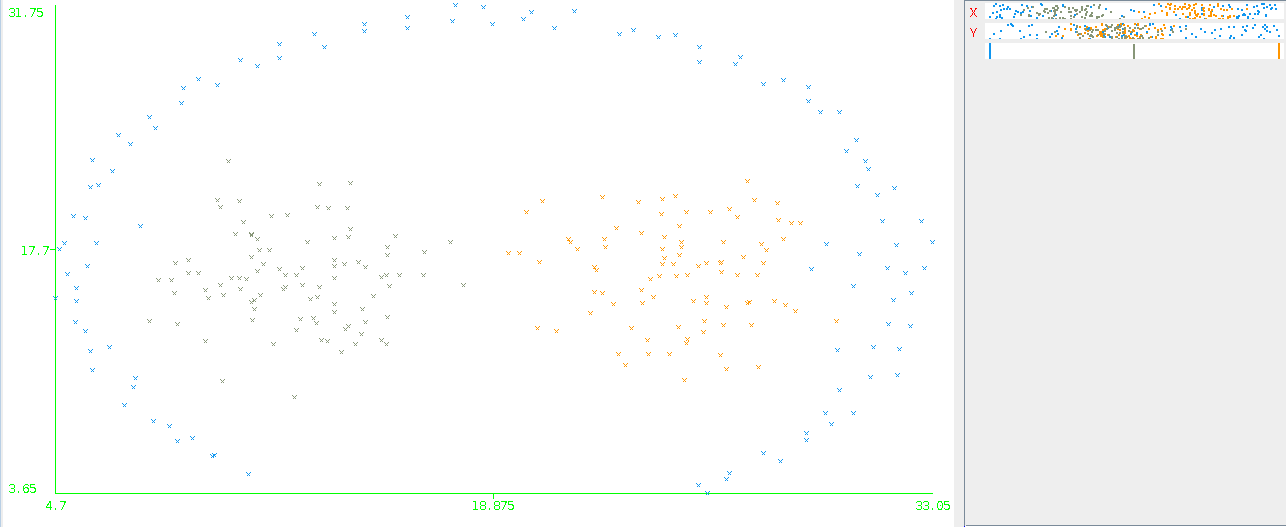
\includegraphics[scale = 0.4]{/home/sneha/Acads/9thsem/ML/P3/path-based.png}
	\caption{Path-based}
	
\end{figure}



\begin{figure}
	\centering
		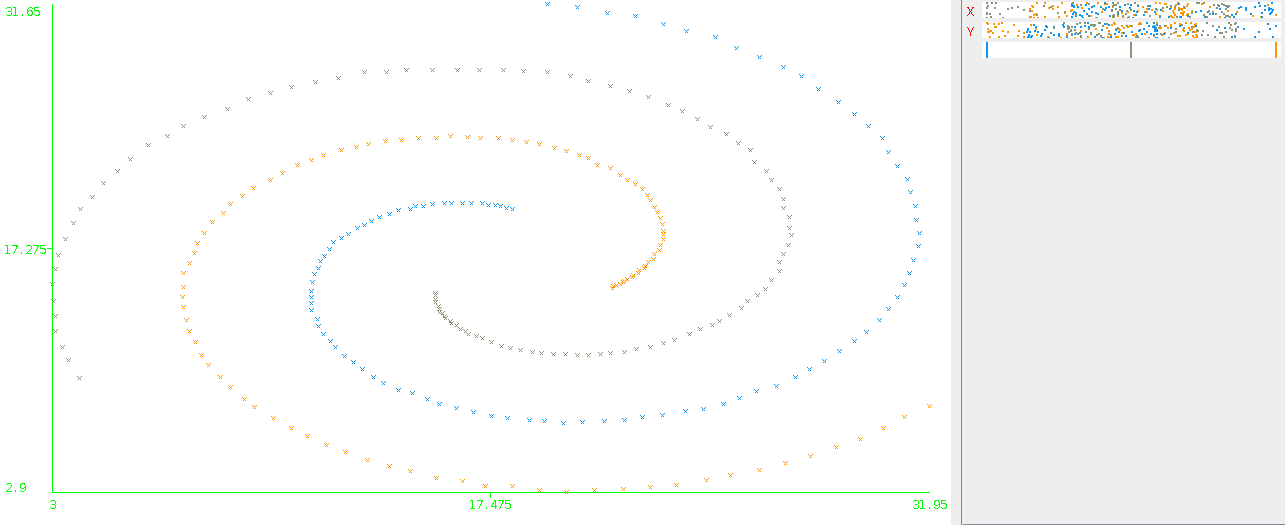
\includegraphics[scale = 0.4]{/home/sneha/Acads/9thsem/ML/P3/spiral.png}
	\caption{Spiral}
	
\end{figure}







}

\item{
K means is run on the R15 cluster with the number of clusters set as 15 and k value set as 8. Out of 599 instances of the data, 114 are incorrectly classified, giving rise to 19\% error in clustering. The graph of k vs cluster purity is given in Figure 8.
\begin{equation}
Cluster Purity = percentage\ of\ instances\ classified\ correctly = 80.97\%
\end{equation}
\begin{figure}
	\centering
		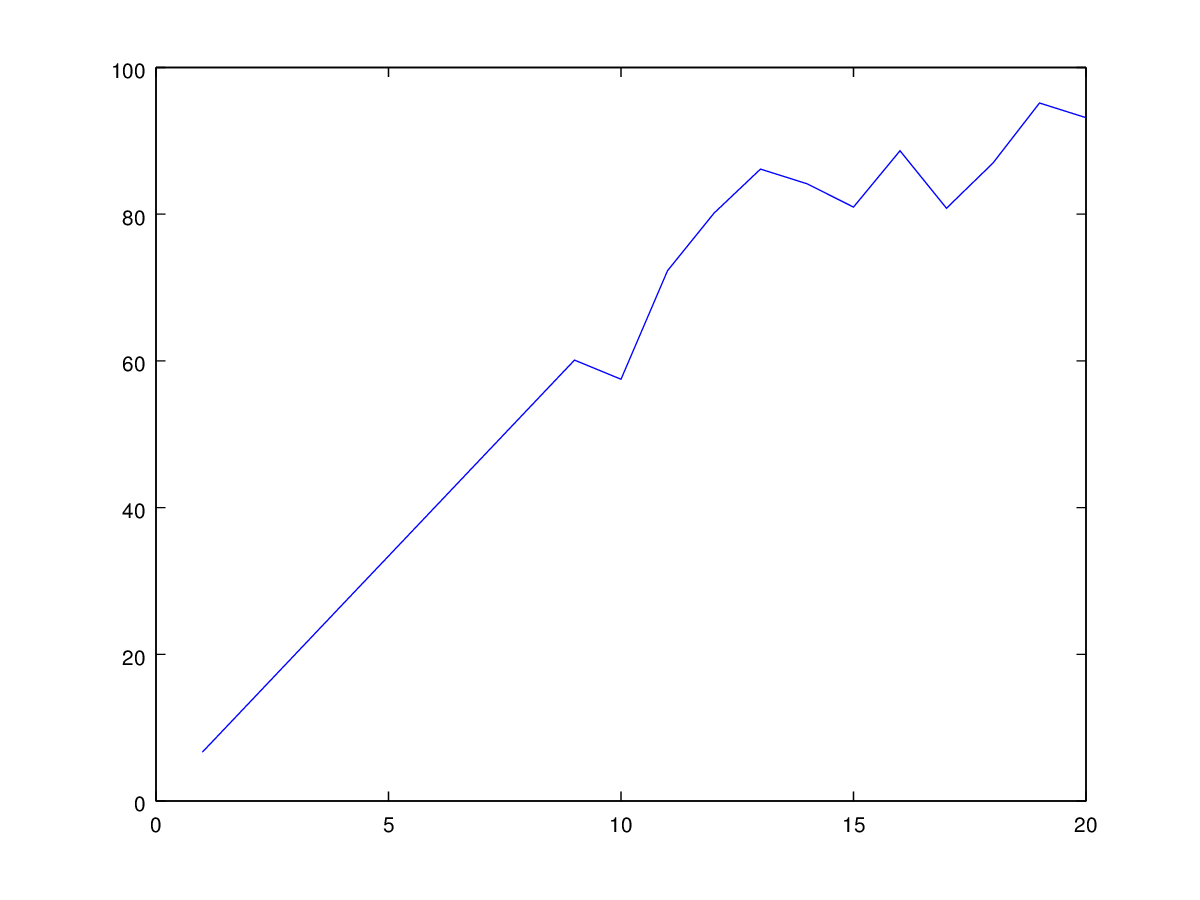
\includegraphics[scale = 0.6]{/home/sneha/Acads/9thsem/ML/P3/p31.png}
	\caption{k vs Cluster purity}
	
\end{figure}

}

\item{
DBSCAN is run on the Jain dataset with minpoints set as 20 and epsilon set as 0.1. 3 instances out of the total 372 instances are incorrectly classified, giving rise to 0.8\% error in the clustering.
\begin{equation}
Cluster Purity = percentage\ of\ instances\ classified\ correctly = 99.2\%
\end{equation}

With decrease in minpoints the cluster purity decreases. Increase in epsilon as well as its decrease from the said optimal point decreases the cluster purity.
}


\item{Comparison of DBSCAN and heirarchical clustering for different datasets is shown in Table 1.
\begin{table}
\centering
		\begin{tabular}{|l | r| c|}
			\hline
		\textbf{Dataset} & \textbf{DBSCAN} & \textbf{Heirarchical} \\ \hline
			 Path-based &  98 & Ward linkage - 75.6 \\ \hline
			Spiral & 100  & Single linkage - 100\\ \hline
			Flames & 99.2 & Ward linkage - 99.2  \\ \hline
			
			
		\end{tabular}
	\caption{Comparision of DBSCAN and Heirarchicals}

\end{table}
}




\end{itemize}


\section{Decision trees}
\begin{itemize}
\item{
The J48 Decision tree algorithm is highly accurate and is giving a precision, recall and f-measure for Minobjects set as 5. 

}
\item{
As the MinObjects increase, precision of one class decreases and the recall of the other class decreases.


}
\item {
The most important feature is the bruises.If there are bruises (f) then the mushroomn is poisonous and if there are no bruises (t) mushroom is edible.
}

\item{ The Decision tree learnt by the model is given in the figure 9.
\begin{figure}
	\centering
		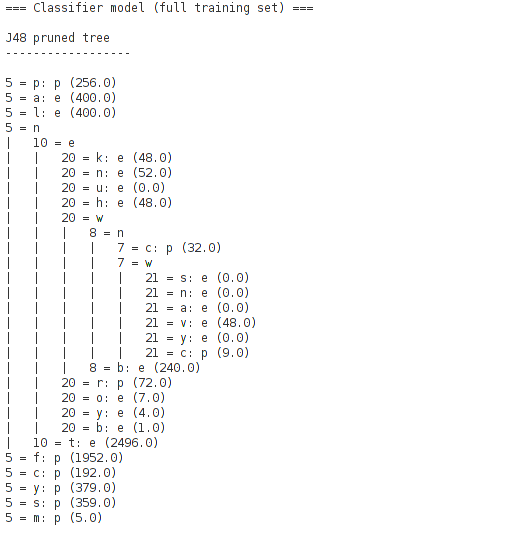
\includegraphics[scale = 0.6]{/home/sneha/Acads/9thsem/ML/P3/mod1.png}
	\caption{Training data model	}
	
\end{figure}

}
\end{itemize}















% --------------------------------------------------------------
%     You don't have to mess with anything below this line.
% --------------------------------------------------------------
 
\end{document}